\documentclass[12pt]{article}
\listfiles
\usepackage[LGR,T1]{fontenc} % Fonts LGR, T1 τα default https://latexref.xyz/fontenc-package.html
\usepackage[utf8]{inputenc} % Encoding γραμματων για τα ελληνικά
\usepackage[margin=12mm]{geometry} % Γεωμετρία εγγράφου (περιθώρια κλπ)

\usepackage{simplehwgr}

% Τιτλοφόρηση
\title{ ΤΙΤΛΟΣ \\ \vspace{10pt}\small{ΥΠΟΤΙΤΛΟΣ}}
\author{Όνομα Επώνυμο \\ Ίδρυμα, Αριθμός Μηρώου\\ \texttt{\href{mailto:email@email.com}{\textlatin{email@email.com}}}}
\date{ΗΜΕΡΟΜΗΝΙΑ}
\setcounter{tocdepth}{3} % Το βάθος των περιεχομένων 5->subparagraph και για figures/tables
%----------------------------------------------------------------------------------------------------------------------%

\begin{document}

\pagenumbering{roman} % Αρχικά αρίθμηση με i,ii
\begin{titlingpage}
\maketitle
\end{titlingpage}
\tableofcontents
\pagebreak
%----------------------------------------------------------------------------------------------------------------------%
\pagenumbering{arabic} % Κανονική αρίθμηση από εδώ και πέρα
%\addcontentsline{toc}{section}{Τμήμα 1}  % Για εισαγωγή (sub)section*{} στο TOC
\section{Παρουσίαση Μαθηματικών Τύπων}

\begin{gather*}
    \mathbb{E}[r_t] = exp[-\beta t]r_0 +\frac{\alpha}{\beta} \left(1 - exp[-\beta t]\right) + \sigma \cancelto{\mathbb{E}[I_t] = 0}{\mathbb{E}\left[\int_0^t \exp[\beta (s-t)] dW_s\right]}  \Rightarrow\\
    \mathbb{E}[r_t] = exp[-\beta t]r_0 +\frac{\alpha}{\beta} \left(1 - exp[-\beta t]\right) \\
    \text{και} \\
    \textlatin{Var}[r_t]=\textlatin{Var}\left[exp[-\beta t]r_0 +\frac{\alpha}{\beta} \left(1 - exp[-\beta t]\right) + \sigma \int_0^t \exp[\beta (s-t)] dW_s \right] \Rightarrow\\ 
    \textlatin{Var}[r_t]=\textlatin{Var}[ \sigma \int_0^t \exp[\beta (s-t)] dW_s ] \Rightarrow\\
    \textlatin{Var}[r_t]=  \sigma^2 \textlatin{Var}[\int_0^t  \exp[\beta (s-t)] dW_s ] = \sigma^2 \int_0^t \exp[2\beta (s-t)] dW_s \Rightarrow \\
    \textlatin{Var}[r_t]=  \sigma^2 \frac{1}{2\beta} (1 - \exp[-2\beta t])
\end{gather*}

\begin{equation}\label{gt}
    g(t)=f(t|>t_0)=\begin{cases}\alpha \cfrac{{t_0}^\alpha}{t^{\alpha +1}} &,t\ge \theta \\ 0 &,t<\theta\end{cases} 
\end{equation}

$$\mathbb{E}\left[T|T>t_0\right]=\int_{t_0}^{\infty}{tg(t)dt}\overset{\eqref{gt}}{=}\int_{t_0}^{\infty}{t\alpha\cfrac{{t_0}^\alpha}{t^{\alpha +1}}dt}=\alpha {t_0}^{\alpha} \int_{t_0}^{\infty}{\cfrac{1}{t^\alpha}dt}=$$
$$=\alpha {t_0}^{\alpha} \left[\cfrac{1}{1 - \alpha} \cfrac{1}{t^{\alpha -1}} \right]^{\infty}_{t_0}=\cfrac{\alpha}{1 - \alpha}{t_0}^{\alpha} \left(-\cfrac{1}{{t_0}^{\alpha -1}}\right)\Rightarrow$$

\begin{align*}
    &\hat{(\alpha,\beta)}_{1,1}=-0.2778 &\hat{(\alpha,\beta)}_{2,1}=-0.6111\hspace{50pt} &\hat{(\alpha,\beta)}_{3,1}=0.8889\\
    &\hat{(\alpha,\beta)}_{2,1}=1.0556 &\hat{(\alpha,\beta)}_{2,2}=0.7222   \hspace{50pt} &\hat{(\alpha,\beta)}_{3,2}=-1.7778\\
    &\hat{(\alpha,\beta)}_{3,1}=-0.7778 &\hat{(\alpha,\beta)}_{2,3}=-0.1111 \hspace{50pt} &\hat{(\alpha,\beta)}_{3,3}=0.8889\\
\end{align*}


\section{Παραδείγματα}
\subsection{\textlatin{Block} κώδικα δίπλα δίπλα }

\begin{otherlanguage}{english}

\begin{minipage}{0.45\linewidth}
\begin{lstlisting}[escapechar=\%]
> model.tables(mod_new,"means") 
Tables of means
Grand mean
         
30.92593 
 malako 
malako
    1     2     3 
29.59 30.93 32.26 
 sklhro 
sklhro
    1     2     3 
28.67 32.67 31.44 
 poikilia 
poikilia
    1     2     3 
32.41 33.52 26.85 
 malako:sklhro 
      sklhro
malako 1     2     3    
     1 25.11 32.00 31.67
     2 29.56 33.56 29.67
     3 31.33 32.44 33.00
\end{lstlisting}
\end{minipage}\hfill
\begin{minipage}{0.45\linewidth}
\begin{lstlisting}
> model.tables(mod_new,"effects") 
Tables of effects
 malako 
malako
      1       2       3 
-1.3333  0.0000  1.3333 
 sklhro 
sklhro
      1       2       3 
-2.2593  1.7407  0.5185 
 poikilia 
poikilia
     1      2      3 
 1.481  2.593 -4.074 
 malako:sklhro 
      sklhro
malako 1       2       3      
     1 -2.2222  0.6667  1.5556
     2  0.8889  0.8889 -1.7778
     3  1.3333 -1.5556  0.2222
\end{lstlisting}
\end{minipage}
\end{otherlanguage}

\selectlanguage{english}
\noindent\begin{minipage}{.45\textwidth}
\begin{lstlisting}
    > AIC(mod_weib_A)
	    [1] 115.303
    > AIC(mod_lognorm_A)
	    [1] 115.4745
    > AIC(mod_loglogistic_A)
	    [1] 115.8543
\end{lstlisting}
\end{minipage}\hfill
\noindent\begin{minipage}{.45\textwidth}
\begin{lstlisting}
    > AIC(mod_weib_B)
	    [1] 71.50213
    > AIC(mod_lognorm_B)
	    [1] 70.88508
    > AIC(mod_loglogistic_B)
	    [1] 71.33654
\end{lstlisting}
\end{minipage}
\noindent\begin{minipage}{.45\textwidth}
\begin{lstlisting}
    > AIC(mod_weib_C)
	    [1] 99.4842
    > AIC(mod_lognorm_C)
	    [1] 95.16805
    > AIC(mod_loglogistic_C)
	    [1] 95.06954
\end{lstlisting}
\end{minipage}\hfill
\noindent\begin{minipage}{.45\textwidth}
\begin{lstlisting}
     > AIC(mod_weib)
     	[1] 292.4813
     > AIC(mod_lognorm)
        [1] 286.2316
     > AIC(mod_loglogistic)
    	[1] 285.9799
\end{lstlisting}
\end{minipage}
\selectlanguage{greek}

\subsection{Πινακάκια}
\subsubsection{\texten{Stylized}}
\begin{tcolorbox}[title=\textlatin{Eulerian} Γράφημα]
\textlatin{Eulerian} γράφημα ονομάζεται αυτό που περιέχει περιήγηση (δηλ. περίπατο με ταυτόσημο πρώτο και τελευταίο κόμβο) η οποία περιέχει κάθε ακμή του γραφήματος ακριβώς μια φορα.
\tcblower
\ul{\textbf{Θεώρημα }}{\begin{otherlanguage}{english}\ul{\textbf{Euler}}\end{otherlanguage}  } \footnote{Όχι αυτό, ούτε εκείνο, ένα ακόμα. } : Ένα συνδεδεμένο γράφημα θα έχει περιήγηση \textlatin{Euler} αν και μόνο αν κάθε κόμβος του είναι άρτιου βαθμού.
\end{tcolorbox}

\subsubsection{Απλό}
\begin{tcolorbox}[title =Ορισμοί ισορροπημένης συμβολοσειράς, colback=white,colbacktitle=white,arc=0mm]
Μια συμβολοσειρά $w \in \{(,)\}^*$ είναι ισορροπημένη \ul{ανν}:
\begin{itemize}
    \item[(α)] 
        \begin{enumerate}
            \item Η $w$ έχει ίσο πλήθος «(» και «)»
            \item Κάθε πρόθεμα της $w$ έχει τουλάχιστον τόσα «(» όσα «)»
        \end{enumerate}
\end{itemize}
    \tcblower
\begin{itemize}
    \item[(β)]
        \begin{enumerate}
                \item H $\epsilon$ είναι ισορροπημένη.
                \item Αν η $w$ είναι ισορροπημένη τότε είναι και η $(w)$.
                \item Αν οι $w, x$ είναι ισορροπημένες τότε είναι και η $wx$.
                \item Τίποτα άλλο δεν είναι ισορροπημένη συμβολοσειρά.
        \end{enumerate}
\end{itemize}
\end{tcolorbox}
\subsubsection{\texten{Tabular}}
\href{https://www.tablesgenerator.com/latex_tables#}{\textlatin{https://www.tablesgenerator.com/latex\_tables\# }}

\begin{table}[H]
\centering
\begin{otherlanguage}{english}
\begin{tabular}{c|ccccc}
\multirow{2}{*}{\begin{otherlanguage}{greek}\textbf{\textbf{Ημέρα}}\end{otherlanguage}} & \multicolumn{5}{c}{\begin{otherlanguage}{greek}\textbf{\textbf{Χειριστής}}\end{otherlanguage}}                                                                                                                                         \\
                       & \multicolumn{1}{c|}{\textbf{1}}              & \multicolumn{1}{c|}{\textbf{2}}              & \multicolumn{1}{c|}{\textbf{3}}              & \multicolumn{1}{c|}{\textbf{4}}              & \textbf{5}              \\ \hline
\textbf{1}                      & \multicolumn{1}{c|}{A$\alpha$ 19}   & \multicolumn{1}{c|}{B$\beta$ 22}    & \multicolumn{1}{c|}{C$\gamma$ 3}    & \multicolumn{1}{c|}{D$\delta$ 59}   & E$\varepsilon$ 50 \\
\textbf{2}                      & \multicolumn{1}{c|}{B$\gamma$ 11}   & \multicolumn{1}{c|}{C$\delta$ 30}   & \multicolumn{1}{c|}{D$\varepsilon$ 49} & \multicolumn{1}{c|}{E$\alpha$ 40}   & A$\beta$ 18     \\
\textbf{3}                      & \multicolumn{1}{c|}{C$\varepsilon$ 17} & \multicolumn{1}{c|}{D$\alpha$ 50}   & \multicolumn{1}{c|}{E$\beta$ 26}    & \multicolumn{1}{c|}{A$\gamma \ $ 2}    & B$\delta$ 47   \\
\textbf{4}                      & \multicolumn{1}{c|}{D$\beta$ 38}    & \multicolumn{1}{c|}{E$\gamma$ 20}   & \multicolumn{1}{c|}{A$\delta$ 29}   & \multicolumn{1}{c|}{B$\varepsilon$ 38} & C$\alpha$ 19   \\
\textbf{5}                      & \multicolumn{1}{c|}{E$\delta$ 41}   & \multicolumn{1}{c|}{A$\varepsilon$ 30} & \multicolumn{1}{c|}{B$\alpha$ 29}   & \multicolumn{1}{c|}{C$\beta \ $ 6}     & D$\gamma$ 22  
\end{tabular}
\end{otherlanguage}
\captionsetup{justification=centering,margin=2cm}
\caption{Δεδομένα επιρροής μεθόδων κατασκευής (λατινικά γράμματα),ημερών (γραμμές), χειριστών (στήλες) και μηχανών (ελληνικά γράμματα) στον αριθμό κατασκευασμένων κομματιών ανά ημέρα.}
\end{table}

\pagebreak
\subsection{Γραφήματα, εικόνες}

\begin{figure}[!h]
\centering
\fbox{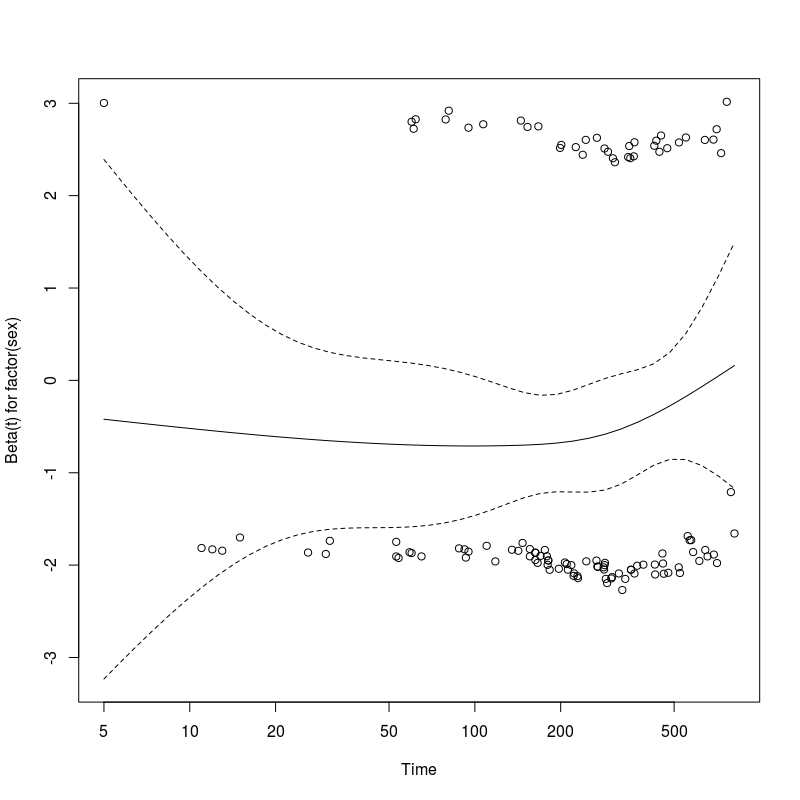
\includegraphics[width=0.5\linewidth]{img/sho2.png}}
\end{figure}
\begin{figure}[!h]
    \centering
    \fbox{
    \begin{subfigure}[b]{0.3\textwidth}
        \centering
        \raisebox{15mm}{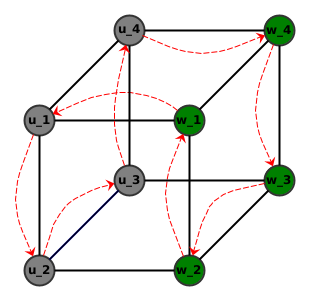
\includegraphics[width=\linewidth]{img/GraphTh_ex1_6.png}}
    \end{subfigure}
    \begin{subfigure}[b]{0.63\linewidth}
        \centering
        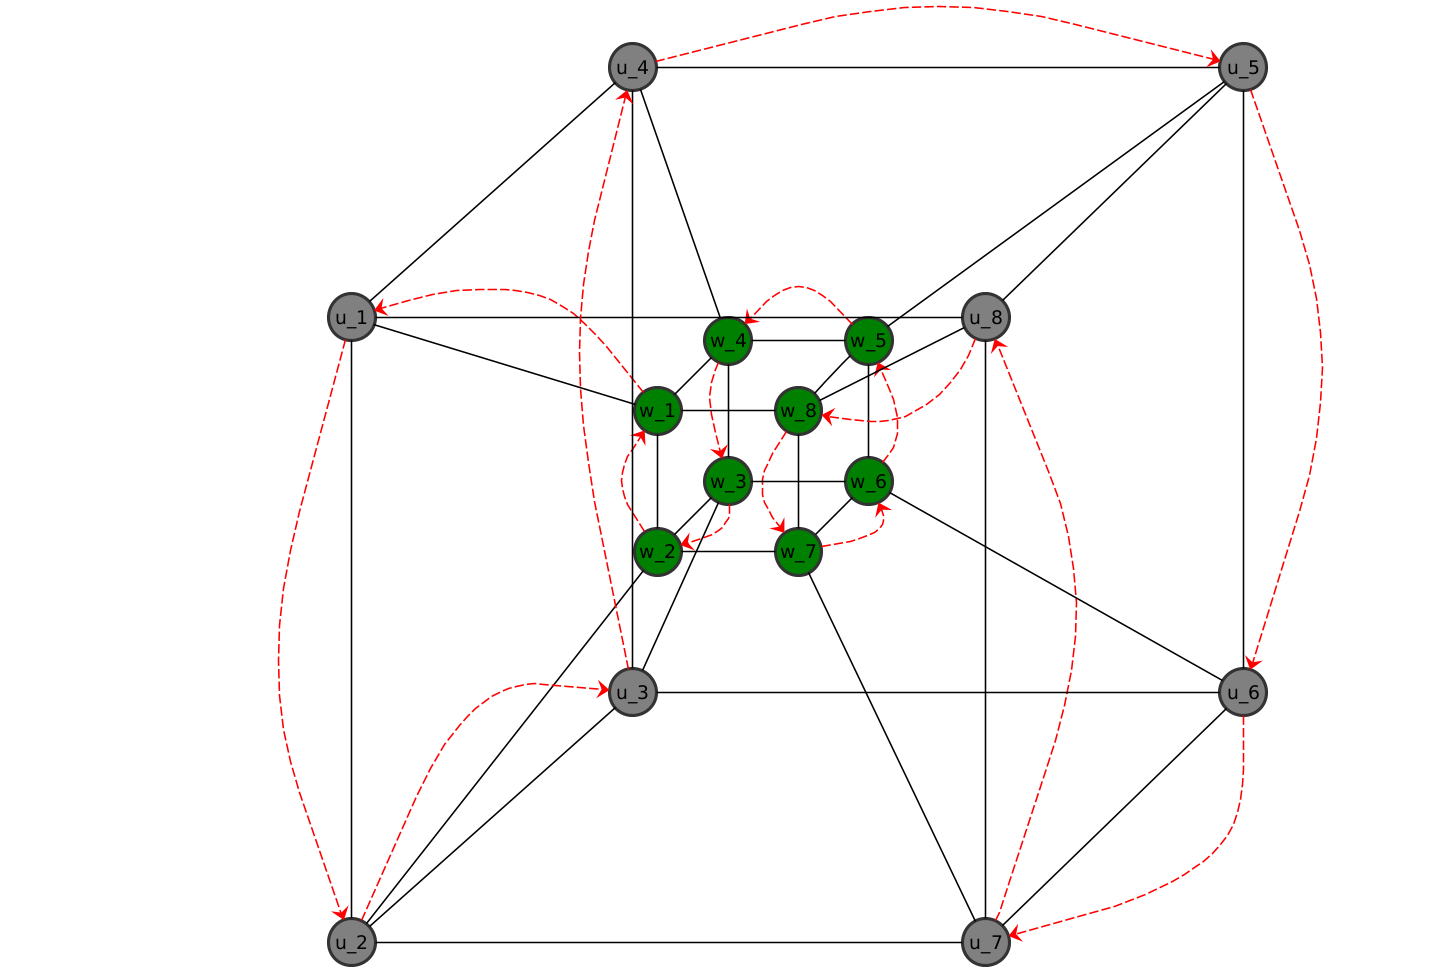
\includegraphics[width=\linewidth]{img/GraphTh_ex1_6_2.png}
    \end{subfigure}
    }
    \caption{Ο \textlatin{Hamiltonian} κύκλος, όπως τον περιγράψαμε, στον $Q_n \text{ για } n=3,4$}
    \label{fig: Qn cycle}
\end{figure}
\newpage
\listoffigures

\listoftables

\end{document}   
